% 第4章第1节：随机变量族与样本路径（共同概率空间、两种读法、有限维分布、路径规律）。

\section{随机变量族与样本路径}
\label{sec:spp-families-paths}

本节确定研究对象。我们从几种重复读数出发，说明为什么一族随机变量必须定义在同一个概率空间上；再分别固定索引和固定一次实现，得到随机变量与样本路径这两种读法。随后用相同边缘、不同相关的序列说明单时刻分布为何不够，引入有限维分布，并把整条路径看成函数空间中的随机元素，检查哪些关于路径的问题可以在这个框架中提出。

\subsection{索引、状态与共同概率空间}
\label{sec:spp-index-state-space}

\paragraph{三种重复读数}
设一台传感器反复测量同一个量，第$n$次读数记为$X_n$，测量噪声$\varepsilon_1,\varepsilon_2,\ldots$相互独立，都服从$\mathcal N(0,\sigma^2)$。下面三种模型都产生一列读数。
\begin{enumerate}
  \item 独立读数：被测量是固定常数$\theta$，$X_n=\theta+\varepsilon_n$。
  \item 共享背景：被测量$\Theta\sim\mathcal N(0,\tau^2)$本身随机（例如当天的环境条件），与全部噪声独立，$X_n=\Theta+\varepsilon_n$。
  \item 误差累计：仪器每次把新误差叠加到上一次读数上，$S_0=0$，$S_n=\varepsilon_1+\cdots+\varepsilon_n$。
\end{enumerate}
第二种模型中每个$X_n$都服从$\mathcal N(0,\tau^2+\sigma^2)$；若在第一种模型中取$\theta=0$，再把噪声方差换成$\tau^2+\sigma^2$，单次读数的分布就与第二种完全相同。只看一次读数，无法区分这两种情形。

区别出现在涉及多次读数的问题上。在共享背景模型中，$\operatorname{Cov}(X_m,X_n)=\tau^2$对$m\ne n$成立，前$n$次读数的平均满足
\[
  \operatorname{Var}\Bigl(\frac1n\sum_{i=1}^nX_i\Bigr)=\tau^2+\frac{\sigma^2}{n},
\]
无论读多少次，平均值的方差都不低于$\tau^2$；而独立读数的平均方差$(\tau^2+\sigma^2)/n$随$n$趋于零。累计模型中$\operatorname{Cov}(S_m,S_n)=\sigma^2\min(m,n)$，相邻读数共享此前的全部误差。这些量都同时涉及第$m$次与第$n$次读数，所以“第$m$次读数”和“第$n$次读数”必须是同一次实验结果$\omega$的两个函数：只有这样，$\{X_1>0,\ X_2>0\}$才是一个有意义的事件。若只给出每次读数各自的分布，就无法回答两次读数是否共享$\Theta$。

\paragraph{随机过程的定义}
因此，研究一族读数时，先固定一个概率空间，再把每个读数写成它上面的随机变量。索引不必是测量轮次，也可以是连续时间、平面上的位置，甚至是可测集合；取值也不必是实数。下面的定义只要求每个坐标可测。

\begin{definition}[随机过程]
\label{def:spp-process}
设$(\Omega,\mathcal F,\mathbb P)$是概率空间，$T$是非空集合，$(E,\mathcal E)$是可测空间。若对每个$t\in T$，映射$X_t:\Omega\to E$都是$\mathcal F/\mathcal E$可测的，就称映射族$X=(X_t)_{t\in T}$为定义在$(\Omega,\mathcal F,\mathbb P)$上、以$T$为\term{索引集}、以$E$为\term{状态空间}的\term{随机过程}（stochastic process）。$T\subseteq\mathbb Z$时也称$X$为\term{随机序列}（random sequence）。
\end{definition}

每个坐标的可测性保证单个读数有分布：$\mathbb P(X_t\in B)$对每个$B\in\mathcal E$有定义，$\mathbb P\circ X_t^{-1}$是$E$上的概率测度。随机对象、推前测度与联合分布的一般讨论可参考\BookChapterRef{chap:probability-models}{卷二“一般概率模型与随机对象”章}；本章需要的只是：同一概率空间上的有限个可测映射$(X_{t_1},\ldots,X_{t_m})$合起来仍是取值于乘积空间$(E^m,\mathcal E^{\otimes m})$的可测映射，因而有联合分布。

几个常见索引可以帮助辨认这个定义的范围。$T=\mathbb N_0$时，$X$是按整数时刻记录的序列；$T=[0,\infty)$时，$X$在每个实数时刻都有值；$T$为平面区域$D$时，$(X_x)_{x\in D}$是一个随机场，例如一片区域上同一时刻的气温；$T$为可测集合族$\mathcal E$时，$(G(A))_{A\in\mathcal E}$可以是一族随机质量，第~\ref{sec:spp-random-measures}节研究的随机概率测度就属于这一类。

\paragraph{固定索引与固定结果}
随机过程是两个变量的函数$(t,\omega)\mapsto X_t(\omega)$，固定其中任何一个都得到有用的对象。固定$t$，得到随机变量$\omega\mapsto X_t(\omega)$，它描述时刻$t$的读数在各次实验之间怎样变化；固定$\omega$，得到一个从$T$到$E$的普通函数。

\begin{definition}[样本路径]
\label{def:spp-sample-path}
对随机过程$X=(X_t)_{t\in T}$和固定的$\omega\in\Omega$，函数$t\mapsto X_t(\omega)$称为$X$的一条\term{样本路径}（sample path），记作$X_\cdot(\omega)$。它是函数集合$E^T=\{x:T\to E\}$中的一个元素。
\end{definition}

图~\ref{fig:spp-two-views}把这两种读法画在一起。左图中每条灰线是一次实验的完整记录，蓝线是其中一条；沿横轴看一条线，读到的是一次实现随时间怎样变化。竖虚线固定一个时刻，它与各条路径的交点是该时刻在不同实验中的读数；把$2000$条路径在两个时刻的交点做成直方图，就得到右图中$S_{10}$与$S_{30}$的分布。竖切片越往后越宽，这是方差$\operatorname{Var}(S_n)=n$的直观形态；但右图的两个直方图没有记录同一条路径在两个时刻的值怎样配对，这部分信息只能沿横向读出。

\begin{figure}[htbp]
  \centering
  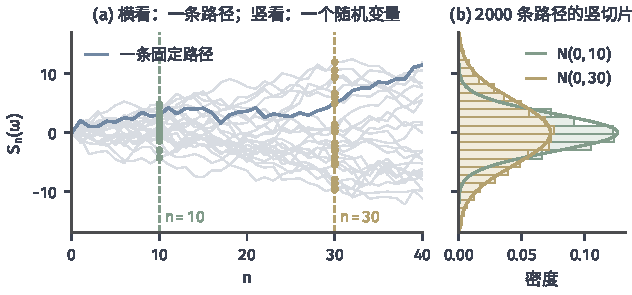
\includegraphics[width=107mm]{figures/03-optimization-evolution-and-signals/02-processes-and-trajectory-evolution/matplotlib/spp-two-views/figure.pdf}
  \caption{随机过程的两种读法。模型为高斯随机游走$S_0=0$，$S_n=\xi_1+\cdots+\xi_n$，$\xi_i$独立服从$\mathcal N(0,1)$，共模拟$2000$条路径（固定随机种子）。(a)灰线为其中$24$条路径，蓝线为一条固定路径；竖虚线固定时刻$n=10$与$n=30$，圆点为前$25$条路径在这两个时刻的值。(b)全部$2000$条路径在这两个时刻的直方图，曲线为精确分布$\mathcal N(0,10)$与$\mathcal N(0,30)$。}
  \label{fig:spp-two-views}
\end{figure}

\begin{example}[三次抛硬币的两种读法]
\label{ex:spp-three-coins}
抛一枚均匀硬币三次，$\Omega=\{\mathrm H,\mathrm T\}^3$，八个结果等可能。令正面记$+1$、反面记$-1$，$\xi_k(\omega)$为第$k$次的记号，$S_0=0$，$S_n=\xi_1+\cdots+\xi_n$，$n=1,2,3$。固定$\omega=\mathrm{HTH}$，样本路径是$(S_0,S_1,S_2,S_3)=(0,1,0,1)$，这是一个确定的四元数组。固定$n=2$，$S_2$在$\mathrm{HH}*$上取$2$，在$\mathrm{HT}*$与$\mathrm{TH}*$上取$0$，在$\mathrm{TT}*$上取$-2$，其中$*$表示第三次任意；因而$\mathbb P(S_2=2)=\mathbb P(S_2=-2)=1/4$，$\mathbb P(S_2=0)=1/2$。前者回答“这一次发生了什么”，后者回答“在时刻$2$可能发生什么、各有多大概率”。
\end{example}

\paragraph{时间、状态与路径的三个判断}
描述一个过程时，有三个彼此独立的判断。第一，索引是离散还是连续：$T=\mathbb N_0$称为离散时间，$T$为实数区间称为连续时间。第二，状态是离散还是连续：$E$可以是有限集、整数集，也可以是$\mathbb R^d$。第三，在连续时间且状态空间带有拓扑时，样本路径是连续的还是带有跳跃。“连续时间”只说明每个实数时刻都有值，并不说明取值连续，更不说明路径连续。

图~\ref{fig:spp-taxonomy}给出四个代表。(a)的简单随机游走在整数时刻取整数值；(b)的自回归序列$Y_{n+1}=0.8Y_n+0.6\eta_{n+1}$在整数时刻取实数值；(c)的计数路径在每个实数时刻都有值，却只取整数，并在随机时刻跳升$1$；(d)的Brownian路径在连续时间中连续变化，但放大后仍然粗糙。连续时间、实数取值的过程也可以有跳跃，例如在计数过程的每次跳跃处加上一个随机实数幅度；在$\mathbb R^d$上运行的Markov链Monte Carlo算法则是离散时间、连续状态的过程。后两章按时间索引组织，正是因为离散时间与连续时间提出的技术问题不同：前者只涉及可数个时刻，后者要处理不可数个时刻，路径性质和可测性需要额外条件。

\begin{figure}[htbp]
  \centering
  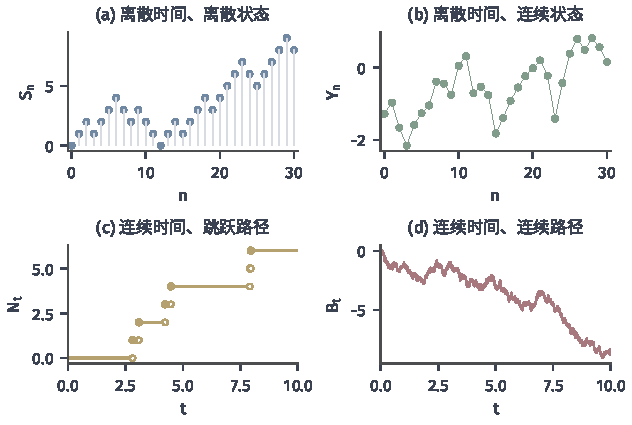
\includegraphics[width=107mm]{figures/03-optimization-evolution-and-signals/02-processes-and-trajectory-evolution/matplotlib/spp-taxonomy/figure.pdf}
  \caption{按索引与路径类型区分的四类过程，均为固定随机种子下的单条模拟路径。(a)简单对称随机游走，每步$\pm1$；(b)平稳自回归序列$Y_{n+1}=0.8Y_n+0.6\eta_{n+1}$，$\eta_n$独立服从$\mathcal N(0,1)$；(c)速率为$1$的计数过程，实心点为跳跃时刻的取值，空心点为跳跃前的左极限；(d)用$4000$个等距小步近似的Brownian路径。时间是离散还是连续，与状态、路径是否连续是分开的判断。}
  \label{fig:spp-taxonomy}
\end{figure}

\subsection{有限维分布与路径规律}
\label{sec:spp-fdd-path-law}

\paragraph{相同边缘、不同依赖}
上一小节的共享背景例子已经说明，单次读数的分布不能决定平均值的行为。下面把这个现象做成一个干净的对照：三个序列的每个坐标都服从$\mathcal N(0,1)$，只有依赖结构不同。取$\rho=0.8$，令$\varepsilon_n,\eta_n,\Theta$均为相互独立的标准高斯变量。
\begin{enumerate}
  \item 独立序列：$X_n=\varepsilon_n$，$\operatorname{Cov}(X_m,X_n)=0$，$m\ne n$。
  \item 自回归序列：$Y_0=\varepsilon_0$，$Y_{n+1}=\rho Y_n+\sqrt{1-\rho^2}\,\eta_{n+1}$。由归纳，$\operatorname{Var}(Y_{n+1})=\rho^2+(1-\rho^2)=1$，且$\operatorname{Cov}(Y_n,Y_{n+k})=\rho^k$。
  \item 共享背景序列：$Z_n=\sqrt\rho\,\Theta+\sqrt{1-\rho}\,\varepsilon_n$，$\operatorname{Var}(Z_n)=\rho+(1-\rho)=1$，$\operatorname{Cov}(Z_m,Z_n)=\rho$，$m\ne n$。
\end{enumerate}
三个序列在任何单个时刻都无法区分。前$100$项平均的方差却分别为
\begin{align*}
  \text{独立序列：}\quad&\frac1{100}=0.01,\\
  \text{自回归序列：}\quad&\frac1{100^2}\Bigl(100+2\sum_{k=1}^{99}(100-k)\rho^k\Bigr)\approx0.086,\\
  \text{共享背景序列：}\quad&\rho+\frac{1-\rho}{100}=0.802 .
\end{align*}
第二个数来自把$\operatorname{Var}(\sum_iY_i)=\sum_{i,j}\rho^{|i-j|}$按间隔$k=|i-j|$分组。图~\ref{fig:spp-same-marginals}显示了差别的来源：独立序列在灰带内来回跳动；自回归序列有记忆，相关随间隔几何衰减；共享背景序列整条路径围绕一个随机水平波动，任意两项的相关都是$0.8$，这个水平不会因为多读几次而被平均掉。

\begin{figure*}[htbp]
  \centering
  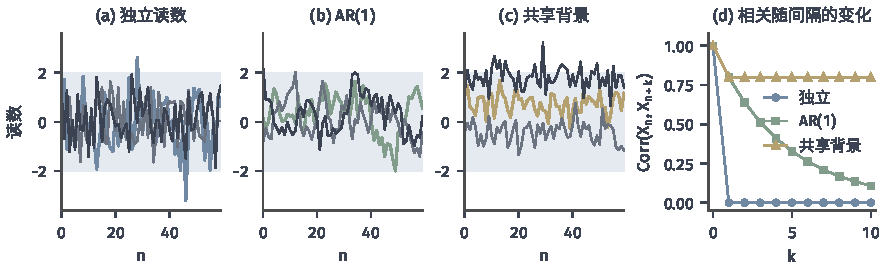
\includegraphics[width=150mm]{figures/03-optimization-evolution-and-signals/02-processes-and-trajectory-evolution/matplotlib/spp-same-marginals/figure.pdf}
  \caption{三个单时刻边缘都为$\mathcal N(0,1)$的序列。(a)--(c)各画三条长$60$的模拟路径（固定随机种子），浅蓝带为$\pm2$，即单个$\mathcal N(0,1)$读数约$95\%$的范围：(a)独立序列；(b)自回归序列，$\rho=0.8$；(c)共享背景序列，$Z_n=\sqrt{0.8}\,\Theta+\sqrt{0.2}\,\varepsilon_n$。(d)理论相关系数随间隔$k$的变化：独立序列在$k\ge1$时为$0$，自回归序列为$0.8^k$，共享背景序列恒为$0.8$。三者前$100$项平均的方差依次为$0.01$、约$0.086$与$0.802$。}
  \label{fig:spp-same-marginals}
\end{figure*}

\paragraph{有限维分布}
要区分这三个序列，至少需要记录任意几个时刻的联合分布。对一般过程，这就是下面的定义。

\begin{definition}[有限维分布]
\label{def:spp-fdd}
设$X=(X_t)_{t\in T}$是取值于$(E,\mathcal E)$的随机过程。对每个正整数$m$和互不相同的$t_1,\ldots,t_m\in T$，令
\[
  \mu_{t_1,\ldots,t_m}(B)=\mathbb P\bigl((X_{t_1},\ldots,X_{t_m})\in B\bigr),\qquad B\in\mathcal E^{\otimes m}.
\]
全体这样的概率测度称为$X$的\term{有限维分布}（finite-dimensional distributions）。
\end{definition}

上面三个序列的有限维分布都是均值为零的高斯分布，区别只在协方差矩阵：独立序列为单位矩阵，自回归序列的$(i,j)$元为$\rho^{|t_i-t_j|}$，共享背景序列的非对角元全为$\rho$。

同一过程的有限维分布不能随意指定，它们之间有两条必然的关系。设$\pi$是$\{1,\ldots,m\}$的一个排列，记$\sigma_\pi(x_1,\ldots,x_m)=(x_{\pi(1)},\ldots,x_{\pi(m)})$。

\begin{theorem}[有限维分布的相容关系]
\label{thm:spp-fdd-consistency}
任意随机过程的有限维分布满足：
\begin{enumerate}
  \item 重排相容：$\mu_{t_{\pi(1)},\ldots,t_{\pi(m)}}=\mu_{t_1,\ldots,t_m}\circ\sigma_\pi^{-1}$；
  \item 边缘相容：对$m\ge2$与$B\in\mathcal E^{\otimes(m-1)}$，$\mu_{t_1,\ldots,t_m}(B\times E)=\mu_{t_1,\ldots,t_{m-1}}(B)$。
\end{enumerate}
\end{theorem}

\begin{proof}
两条都是同一个事件的两种写法。对$B\in\mathcal E^{\otimes m}$，$(X_{t_{\pi(1)}},\allowbreak\ldots,\allowbreak X_{t_{\pi(m)}})\in B$当且仅当$(X_{t_1},\allowbreak\ldots,\allowbreak X_{t_m})\in\sigma_\pi^{-1}(B)$，两边取概率即得第一条。$(X_{t_1},\allowbreak\ldots,\allowbreak X_{t_m})\in B\times E$当且仅当$(X_{t_1},\allowbreak\ldots,\allowbreak X_{t_{m-1}})\in B$，因为最后一个坐标总在$E$中，取概率即得第二条。
\end{proof}

相容关系说的是：同一个“两时刻问题”，不论直接用两时刻分布回答，还是从三时刻分布中积掉第三个坐标再回答，答案必须一样。第~\ref{sec:spp-kolmogorov-extension}小节讨论反方向的问题：给定一族满足这两条的分布，是否一定存在过程以它们为有限维分布。

\paragraph{路径作为随机元素}
有限维分布一次只看有限个时刻。“路径是否曾越过某个水平”这类问题涉及整条路径，需要把路径本身当作一个随机对象。把每个$\omega$映到它的样本路径，得到映射
\[
  X:\Omega\to E^T,\qquad \omega\mapsto X_\cdot(\omega).
\]
要谈论$X$的分布，先要在$E^T$上选定$\sigma$代数。最自然的选择是让每个坐标读取$\pi_t:x\mapsto x(t)$都可测的最小$\sigma$代数，即\term{乘积$\sigma$代数}（product sigma-algebra）$\mathcal E^{\otimes T}$。它也由形如
\begin{equation}
  C=\bigl\{x\in E^T:\ (x(t_1),\ldots,x(t_m))\in B\bigr\},\qquad t_1,\ldots,t_m\in T,\ B\in\mathcal E^{\otimes m}
  \label{eq:spp-cylinder}
\end{equation}
的集合生成，这类集合称为\term{柱集}（cylinder set）：它只在有限个时刻检查路径是否满足某项条件，其余时刻不加限制。图~\ref{fig:spp-cylinder}中三个时刻各设一道“闸门”，柱集就是同时穿过三道闸门的全部路径；闸门之间路径怎样走，柱集不管。

\begin{figure}[htbp]
  \centering
  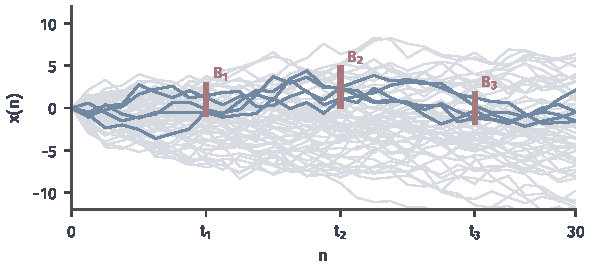
\includegraphics[width=100mm]{figures/03-optimization-evolution-and-signals/02-processes-and-trajectory-evolution/matplotlib/spp-cylinder/figure.pdf}
  \caption{柱集$\{x:\ x(t_1)\in B_1,\ x(t_2)\in B_2,\ x(t_3)\in B_3\}$。红色竖条为三个时刻上的区间$B_1=[-1,3]$、$B_2=[0,5]$、$B_3=[-2,2]$；$60$条高斯随机游走路径（固定随机种子）中，同时穿过三个区间的画成蓝色，其余为灰色。柱集只约束这三个时刻的取值。}
  \label{fig:spp-cylinder}
\end{figure}

\begin{theorem}[路径映射的可测性与路径规律]
\label{thm:spp-path-law}
设$X=(X_t)_{t\in T}$是取值于$(E,\mathcal E)$的一族映射。
\begin{enumerate}
  \item 路径映射$X:(\Omega,\mathcal F)\to(E^T,\mathcal E^{\otimes T})$可测，当且仅当每个$X_t$可测，即$X$是随机过程。
  \item 若$X$是随机过程，则推前测度$P_X=\mathbb P\circ X^{-1}$是$(E^T,\mathcal E^{\otimes T})$上的概率测度，称为$X$的\term{路径规律}（law of the process）。两个随机过程（可以定义在不同的概率空间上）具有相同的有限维分布，当且仅当它们的路径规律相同。
\end{enumerate}
\end{theorem}

\begin{proof}
(1) 由于$\pi_t\circ X=X_t$，若$X$可测，则每个$X_t$作为可测映射的复合可测。反之，若每个$X_t$可测，则$\{B\subseteq E^T:\ X^{-1}(B)\in\mathcal F\}$是$\sigma$代数，并包含每个$\pi_t^{-1}(A)$，因为$X^{-1}(\pi_t^{-1}(A))=X_t^{-1}(A)\in\mathcal F$；它因而包含这些集合生成的$\mathcal E^{\otimes T}$。

(2) 柱集\eqref{eq:spp-cylinder}的概率是$P_X(C)=\mu_{t_1,\ldots,t_m}(B)$，所以路径规律相同蕴含有限维分布相同。反过来，两个柱集的交仍是柱集：把两组时刻合并，各自的条件改写到合并后的坐标上即可。于是柱集族是对有限交封闭、生成$\mathcal E^{\otimes T}$的集合族。两个概率测度若在这样的集合族上相等，就在它生成的$\sigma$代数上相等（这是$\pi$--$\lambda$定理的推论，可参考\BookChapterRef{chap:measures}{卷二“测度”章}）。有限维分布相同意味着两个路径规律在全部柱集上相等，因而处处相等。
\end{proof}

这一定理说明，在乘积$\sigma$代数的层面上，“过程的规律”与“全部有限维分布”是同一份信息。它也划定了这份信息的边界：只有属于$\mathcal E^{\otimes T}$的路径事件，其概率才由有限维分布决定。

\paragraph{可数个坐标决定的事件}
索引可数时，乘积$\sigma$代数已经包含许多关于整条路径的事件。设$T=\mathbb N_0$，$E=\mathbb R$。“路径曾超过$c$”是可数并$\bigcup_n\{x:\ x(n)>c\}$；“路径收敛”可以写成$\{\limsup_nx(n)=\liminf_nx(n)\in\mathbb R\}$，而$\limsup_nx(n)=\inf_m\sup_{n\ge m}x(n)$是可测函数的可数次上下确界。这些事件的概率都由有限维分布决定，第~\ref{chap:discrete-time-stochastic-processes}章研究的回返、命中和极限问题都在这个框架内。

索引不可数时情况不同。关键在于下面的观察：乘积$\sigma$代数中的每个事件只依赖可数个坐标。

\begin{theorem}[乘积$\sigma$代数中的事件由可数个坐标决定]
\label{thm:spp-countable-coordinates}
设$A\in\mathcal E^{\otimes T}$。则存在可数集合$S\subseteq T$，使得对任意$x,y\in E^T$，只要$x$与$y$在$S$上相等，就有$x\in A\Leftrightarrow y\in A$。
\end{theorem}

\begin{proof}
记$\mathcal D$为具有上述性质的集合$A\subseteq E^T$组成的族。柱集\eqref{eq:spp-cylinder}属于$\mathcal D$，取$S=\{t_1,\ldots,t_m\}$即可。若$A\in\mathcal D$，对应可数集$S$，则$A^c$用同一个$S$也满足要求。若$A_k\in\mathcal D$对应$S_k$，令$S=\bigcup_kS_k$，它仍可数；当$x,y$在$S$上相等时，它们在每个$S_k$上相等，于是对每个$k$有$x\in A_k\Leftrightarrow y\in A_k$，从而$x\in\bigcup_kA_k\Leftrightarrow y\in\bigcup_kA_k$。所以$\mathcal D$是包含柱集的$\sigma$代数，含有$\mathcal E^{\otimes T}$。
\end{proof}

取$T=[0,1]$，$E=\mathbb R$。连续函数全体$C[0,1]$不属于$\mathbb R^{\otimes[0,1]}$：若它属于，设对应的可数集为$S$，取$t^\ast\in[0,1]\setminus S$；零函数连续，而函数$\mathbb I_{\{t=t^\ast\}}$与零函数在$S$上相等，却在$t^\ast$处不连续，与定理矛盾。同样的论证表明$\{x:\ \sup_{t\in[0,1]}x(t)>0\}$也不在乘积$\sigma$代数中。因此，对连续时间过程，单凭有限维分布甚至不能提出“路径连续的概率是多少”这个问题。第~\ref{sec:spp-versions}小节将说明怎样通过选取合适的过程版本绕过这一障碍。
